% Template for Cogsci submission with R Markdown

% Stuff changed from original Markdown PLOS Template
\documentclass[10pt, letterpaper]{article}

\usepackage{cogsci}
\usepackage{pslatex}
\usepackage{float}
\usepackage{caption}

% amsmath package, useful for mathematical formulas
\usepackage{amsmath}

% amssymb package, useful for mathematical symbols
\usepackage{amssymb}

% hyperref package, useful for hyperlinks
\usepackage{hyperref}

% graphicx package, useful for including eps and pdf graphics
% include graphics with the command \includegraphics
\usepackage{graphicx}

% Sweave(-like)
\usepackage{fancyvrb}
\DefineVerbatimEnvironment{Sinput}{Verbatim}{fontshape=sl}
\DefineVerbatimEnvironment{Soutput}{Verbatim}{}
\DefineVerbatimEnvironment{Scode}{Verbatim}{fontshape=sl}
\newenvironment{Schunk}{}{}
\DefineVerbatimEnvironment{Code}{Verbatim}{}
\DefineVerbatimEnvironment{CodeInput}{Verbatim}{fontshape=sl}
\DefineVerbatimEnvironment{CodeOutput}{Verbatim}{}
\newenvironment{CodeChunk}{}{}

% cite package, to clean up citations in the main text. Do not remove.
\usepackage{cite}

\usepackage{color}

% Use doublespacing - comment out for single spacing
%\usepackage{setspace}
%\doublespacing


% % Text layout
% \topmargin 0.0cm
% \oddsidemargin 0.5cm
% \evensidemargin 0.5cm
% \textwidth 16cm
% \textheight 21cm

\title{Drawings as a window into object representations in childhood}


\author{{\large \bf Bria Long} \\ \texttt{bria@stanford.edu} \\ Department of Psychology \\ Stanford University \And {\large \bf Judy Fan} \\ \texttt{jefan@stanford.edu} \\ Department of Psychology \\ Stanford University \And {\large \bf Michael C. Frank } \\ \texttt{mcfrank@stanford.edu} \\ Department of Psychology \\ Stanford University}

\begin{document}

\maketitle

\begin{abstract}
The abstract should be one paragraph, indented 1/8 inch on both sides,
in 9 point font with single spacing. The heading Abstract should be 10
point, bold, centered, with one line space below it. This one-paragraph
abstract section is required only for standard spoken papers and
standard posters (i.e., those presentations that will be represented by
six page papers in the Proceedings).

\textbf{Keywords:}
object representations; drawings; child development
\end{abstract}

\section{Introduction}\label{introduction}

(Newell \& Simon, 1972)

Consider what one has to do in order to draw ``a phone'' -- one needs to
access a the mental representation of ``a phone'', distill this into a
pictoral format, and plan a sequence of motor actions to effectively
convey this visual concept. Yet this is a trivial task for ordinary
adults. How do we learn to so effectively produce recognizable drawings?
And might drawings offer a window into how young children represent
common object categories?

While drawing has been extensively studied in early childhood, a primary
focus has been on when children come to treat drawings as symbols for
object categories (Gardner, 1973). And a wealth of evidence now suggests
that in fact young children attribute rich meanings to their drawings.
For example, children will attribute different symbolic content (e.g.,
``a balloon'', ``a lollipop'') to very similar drawings based on what
they intended to draw (Bloom \& Markson, 1998). Further, children will
monitor whether their drawings are adequate symbols for the things they
are trying to draw, and will improve their drawings when given feedback
that their drawings are not effective at communicating the identity of
object (Callagan, 1999).

Far less research, however, has examined how children's drawings reflect
how children represent objects in the world around them. Indeed,
drawings are a powerful way to tap internal representations of object
categories, even in non-expert adults. For example, adults tend to draw
objects that are small in the real-world at small visual sizes, and
objects that are big in the real-world at big visual sizes (Konkle \&
Oliva, 2011). Further, to be recognizable, drawings have to depict the
necessary features to express a given visual concept. This intuition is
supported by recent computational work: deep neural network models of
the ventral stream trained purely on photographs can also recognize
drawings by non-expert adults, as drawings and photographs generated
similar representations in higher-level layers of these models. In other
words, drawings capture high-level similarity relationships between
object categories (Fan, Yamins, \& Turk-Browne, 2015).

Here, we explore how children draw common object categories across early
childhood. First, we ask if children produce more recognizable drawings
as they get older after factoring out low-level covariates (e.g., the
number of strokes, ink used). Second, we examine the degree to which
children's drawings contain the perceptual features characteristic of
common object categories by comparing their representations in a deep
convolutional neural network.

\section{Part 1: How recognizable are drawings across
childhood?}\label{part-1-how-recognizable-are-drawings-across-childhood}

First, we examined how children across a wide range of ages produced
drawings of 16 common object categories in a simple drawing game. Then,
we asked naïve adults to recognize these drawings using a forced-choice
recognition task.

\subsection{Methods}\label{methods}

\subsubsection{Participants.}\label{participants.}

For the drawing task, children (N = 41, M = 6.9 years, range 4-10 years)
were recruited at the San Jose Children's Discovery Museum and
participated in this experiment. For the recognizability experiment, 14
adults with US IP addresses were recruited and rated all of the 268
drawings.

\subsubsection{Materials.}\label{materials.}

We implemented a simple drawing game in HTML/Javascript using the
paper.js library; this web-based experiment was run on an iPad on the
floor of the museum. All code is available at
www.github.com/brialorelle/kiddraw/museumdraw.

\subsubsection{Drawing Game Procedure:}\label{drawing-game-procedure}

On each trial, a text cue would appear (i.e., ``Can you draw a
{[}dog{]}?'') that the experimenter would read out, (``What about a
{[}dog{]}? Can you draw a {[}dog{]}?). Then, a drawing canvas appeared
(600 x 600 pixels) and children were had 30 seconds to make a drawing
before the game moved on to the next trial. After each trial, the
experimenter asked the child whether they wanted to keep drawing or
whether they were all done. On the first two trials of the experiment,
every child was prompted to draw the same two common shapes--- a circle
and a triangle. These trials served to familiarize children with the
drawing task and to practice using their fingers to draw.

\subsubsection{Stimuli.}\label{stimuli.}

Stimuli were words referring to 16 common object categories (banana,
boat, car, carrot, cat, chair, couch, cup, flower, foot, frog, ice
cream, phone, rabbit, shoe, train). These categories were chosen such
that they were (1) likely to be familiar to children, (2) present in the
Google QuickDraw database, (3) spanned the animate/inanimate distinction
and (4) intuitively spanned a wide range of difficulty (for example,
flowers seem easier to draw than couches).

\subsubsection{Recognizability Task:}\label{recognizability-task}

14 naïve adults assessed the recognizability of all of the 286 drawings
produced by these children. On each trial, participants saw a drawing,
and were asked ``What does this look like?'', and responded by typing
into a text box; participants could then choose between 21 possible
answers. 16 of these possible answers were the original object
categories; however, we also included five additional foil items (bean,
arm, person, rock, and ``cannot tell at all''). All drawings were
presented in a random order, and participants were not informed that
these drawings were produced by children or the context in which they
were produced. An answer was scored as ``correct'' if adults were able
to correctly guess the object category that children were cued with.

\subsection{Load data and do basic
preprocessing.}\label{load-data-and-do-basic-preprocessing.}

\begin{CodeChunk}
\begin{CodeOutput}
[1] TRUE
\end{CodeOutput}
\end{CodeChunk}

Number of drawings: 286

Number of drawers: 41

Average age of drawers: 6.9

\subsection{Analysis}\label{analysis}

\begin{CodeChunk}
\begin{figure*}[h]

{\centering 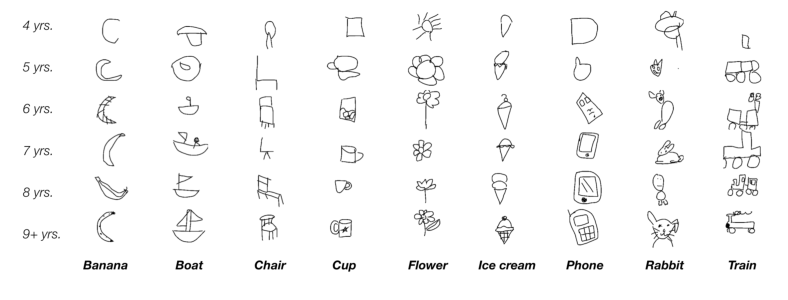
\includegraphics{figs/2-col-image-1} 

}

\caption[This image spans both columns]{This image spans both columns. And the caption text is limited to 0.8 of the width of the document.}\label{fig:2-col-image}
\end{figure*}
\end{CodeChunk}

\subsubsection{Low-level covariates.}\label{low-level-covariates.}

The use of a digital interface for drawing allowed us to quickly and
easily assess the contribution of several low-level factors that may
co-vary with drawing ability. For each drawing, we thus quantified the
amount of time spend drawings, the number of strokes used, and the
overall intensity (e.g., amount of ink). These factors were entered into
the generalized logistic mixed-effect model referenced below.

\begin{CodeChunk}
\begin{figure}[H]

{\centering 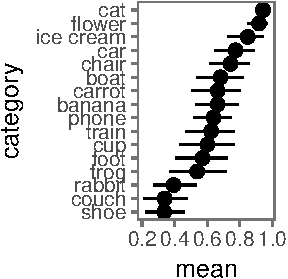
\includegraphics{figs/plot-1} 

}

\caption[R plot]{R plot}\label{fig:plot}
\end{figure}
\end{CodeChunk}

\subsubsection{GLMM procedure.}\label{glmm-procedure.}

We aimed to assess whether children's ability to produce recognizable
drawings increased with age, independent of low-level covariates. To do
so, we used a generalized logistic mixed effect model, with the
following parameters:

\begin{CodeChunk}


               Estimate   Std. Error   z value   Pr(>|z|)
------------  ---------  -----------  --------  ---------
(Intercept)      -2.977        0.755    -3.941          0
age               0.538        0.099     5.427          0

\end{CodeChunk}

\subsection{Results}\label{results}

Overall, we found that the recognizability of children's drawings
increases with the age of the drawer. This can be seen qualitatively in
a set of example drawings in Figure 2, is quantified in Figures 3 and 4.
This relationship persisted even when we accounted for the influence of
several low-level covariates, including the amount of time spent
drawing, the number of strokes used, and the total ``ink'' used
(```\{r\} stats). Interestingly, this relationship held despite the
presence of some items in the dataset that were extremely easy for
children to draw (e.g., flowers; see Figure XX) and some items that were
quite difficult to depict (e.g., couch).

These results also suggest that the ability to produce visual concepts
is highly developed by middle childhood. In under 30 seconds, even
6-year-olds produced drawings that were on average \%\% recognizable in
our 21AFC task.

\subsection{Part 2: Perceptual features of children's drawings across
childhood}\label{part-2-perceptual-features-of-childrens-drawings-across-childhood}

Recognizability ratings may underestimate the perceptual content
depicted in children's drawings. For example, children may not be able
to depict the visual differences between a bunny and a frog, but they
still may capture many of the essential perceptual features needed to
depict an animal. Indeed, this trend was somewhat evident in the
confusion matrices from beforehand: drawings of cats were most confused
with frogs and bunnies (and not couches or chairs). Here, we turn to
deep neural network models of object recognition to quantify the
perceptual features in children's drawings.

Here, we aimed to collect a larger sample of drawings using the same
methodology, this time sampling from both the previously used categories
as well as a new selection of 22 categories (see Stimuli) allowing us to
broadly span superordinate category distinctions. With this broader
sample of drawings, we asked the following questions

\subsection{One-column images}\label{one-column-images}

Single column is the default option, but if you want set it explicitly,
set \texttt{fig.env} to \texttt{figure}. Notice that the
\texttt{num.cols} option for the caption width is set to \texttt{1}.

\begin{CodeChunk}
\begin{figure}[H]

{\centering 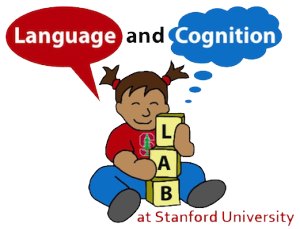
\includegraphics{figs/image-1} 

}

\caption[One column image]{One column image.}\label{fig:image}
\end{figure}
\end{CodeChunk}

\subsection{R Plots}\label{r-plots}

You can use R chunks directly to plot graphs. And you can use latex
floats in the fig.pos chunk option to have more control over the
location of your plot on the page. For more information on latex
placement specifiers see
\textbf{\href{https://en.wikibooks.org/wiki/LaTeX/Floats,_Figures_and_Captions}{here}}

\subsection{Tables}\label{tables}

Number tables consecutively; place the table number and title (in 10
point) above the table with one line space above the caption and one
line space below it, as in Table 1. You may float tables to the top or
bottom of a column, set wide tables across both columns.

You can use the xtable function in the xtable package.

\begin{table}[H]
\centering
\begin{tabular}{rrrrr}
  \hline
 & Estimate & Std. Error & t value & Pr($>$$|$t$|$) \\ 
  \hline
(Intercept) & 0.04 & 0.10 & 0.4 & 0.66 \\ 
  x & 1.95 & 0.11 & 18.4 & 0.00 \\ 
   \hline
\end{tabular}
\caption{This table prints across one column.} 
\end{table}

\section{Acknowledgements}\label{acknowledgements}

Place acknowledgments (including funding information) in a section at
the end of the paper.

\section{References}\label{references}

\setlength{\parindent}{-0.1in} \setlength{\leftskip}{0.125in} \noindent

\hypertarget{refs}{}
\hypertarget{ref-NewellSimon1972a}{}
Newell, A., \& Simon, H. A. (1972). \emph{Human problem solving}.
Englewood Cliffs, NJ: Prentice-Hall.

\end{document}
